\documentclass[11pt]{article}
\usepackage[margin=0.66in]{geometry}
\usepackage{booktabs,enumitem,fancyhdr,graphicx,tabularx,titlesec}
\usepackage[table]{xcolor}
\usepackage[hidelinks]{hyperref}
\graphicspath{{docs/lessons/046/}{./}}
\hypersetup{pdftitle={ADK Lesson 046: Tactile and Directional Intent},
 pdfauthor={Kevin Shanahan},
 pdfsubject={Copied interaction evidence, qualification, and directional hysteresis},
 pdflang={en-US}}
\pagestyle{fancy}\fancyhf{}
\lhead{\textsc{ADK Lesson 046}}\rhead{Tactile and Directional Intent}
\cfoot{\thepage}\setlength{\headheight}{14pt}
\setlength{\parindent}{0pt}\setlength{\parskip}{4pt}
\setlist{nosep,leftmargin=1.45em}
\titleformat{\section}{\Large\bfseries}{\thesection}{0.5em}{}
\newcommand{\lessonbox}[1]{\begin{center}\fbox{\parbox{0.92\linewidth}{#1}}\end{center}}
\newcommand{\blankline}{\rule{0.9in}{0.4pt}}

\begin{document}
\begin{center}
 {\Huge\bfseries Tactile and Directional Intent}\\[4pt]
 {\Large Turn two copied observations into one coherent decision}\\[8pt]
 \fbox{\textbf{E0 COPIED-EVIDENCE REPLAY --- NO POWERED INPUT CLAIM}}
\end{center}
\begin{tabularx}{\linewidth}{@{}>{\bfseries}l X >{\bfseries}l X@{}}
Lesson & 046 --- component & Time & 90--120 minutes\\
Prerequisites & Lessons 031 and 037 & Board & compile-only Mega replay\\
Evidence & named memory result cells & Boundary & no GPIO, ADC, bus, or live clock\\
\end{tabularx}

\lessonbox{\textbf{Responsibility.} Qualify one copied contact action and one
copied directional observation, then publish one age-qualified interaction
snapshot. Preserve both source identities, sequences, statuses, and ages.
Do not infer capacitive sensing, gesture, proximity, pulse, or identity.}

\section{Copy evidence before deriving intent}
\begin{center}
% ADK visual: pencil
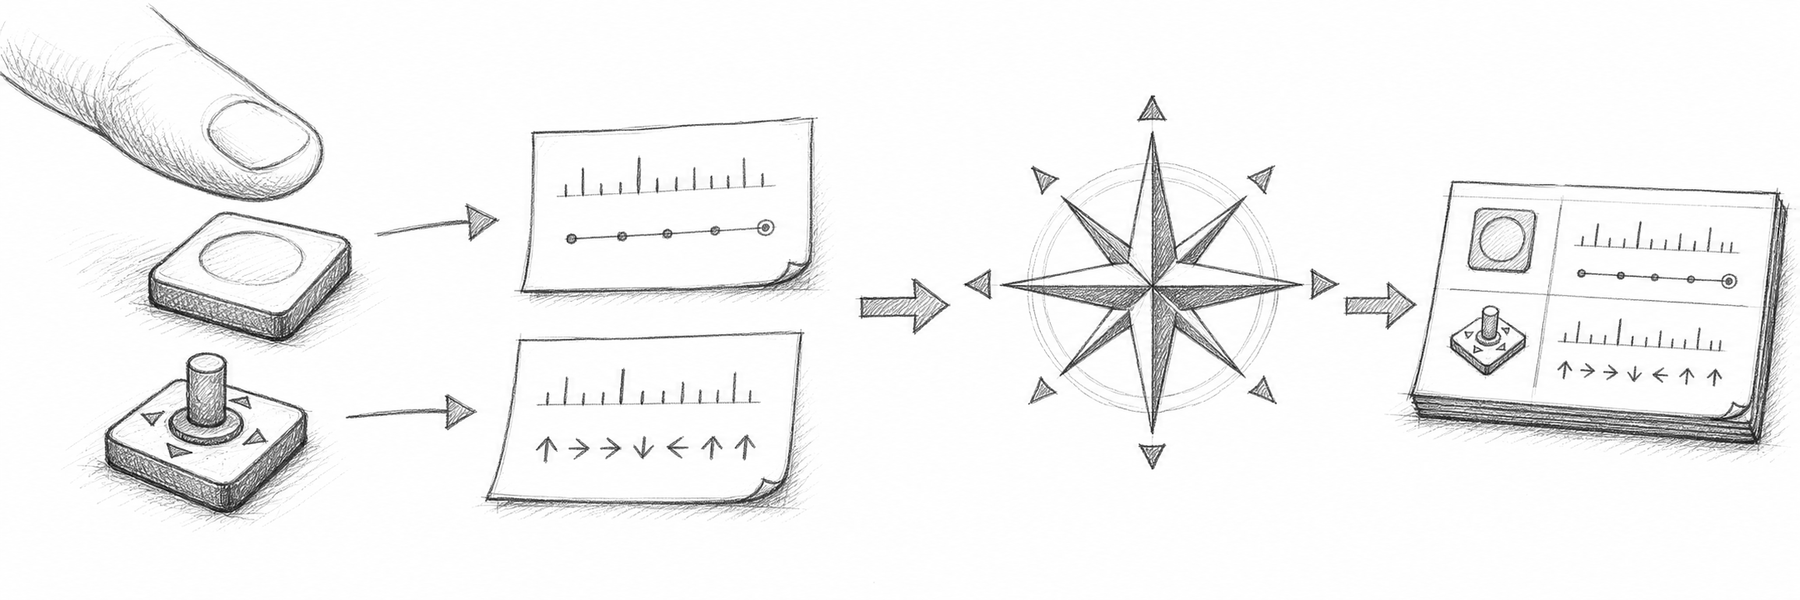
\includegraphics[width=0.98\linewidth,height=0.27\textheight,
 keepaspectratio]{046-copied-intent-pencil.png}

\small\textit{Alternative text: a graphite pencil drawing follows an inert
touch token and directional token into separate copied evidence cards, an
eight-way compass, and one bundled interaction snapshot; no wires or powered
hardware appear.}
\end{center}

\texttt{InteractionIntent\allowbreak Policy} is a narrow facade, not a
universal sensor interface. It privately reuses
\texttt{Contact\allowbreak Dynamics} and derives direction
from already-calibrated axes in permille. The source domain is kind, source
ID, and configuration revision.

\begin{tabularx}{\linewidth}{@{}l X@{}}
\toprule
Copied fact & Why it remains visible\\
\midrule
two source domains & prevents evidence from different producers being confused\\
two timestamps and ages & prevents a fresh joystick from hiding stale contact\\
two sequences & exposes repeats, gaps, regressions, and source changes\\
two producer statuses & prevents either fault from being hidden by the other\\
saturation marker & preserves valid extreme directional evidence\\
\bottomrule
\end{tabularx}

\newpage
\section{Qualify contact; apply directional hysteresis}
\begin{center}
% ADK visual: pencil
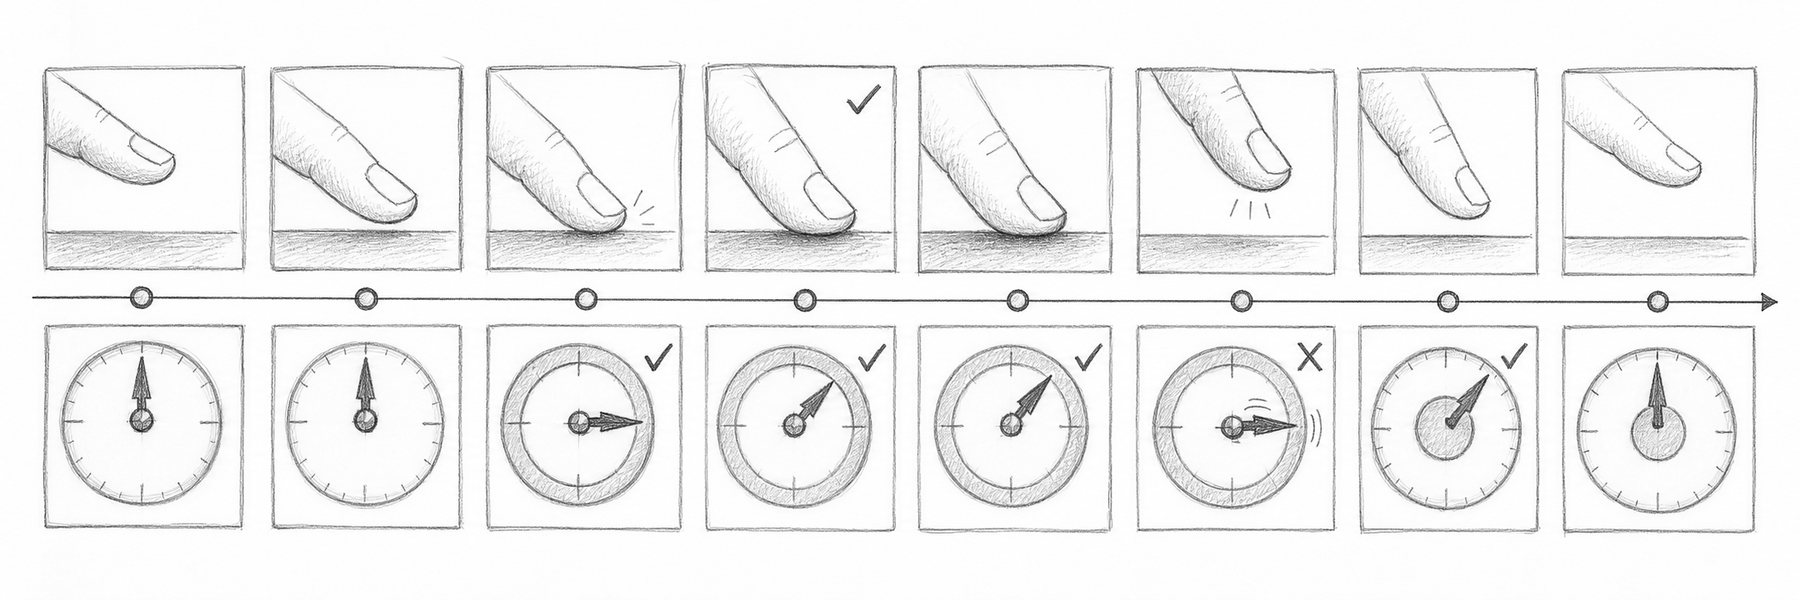
\includegraphics[width=0.98\linewidth,height=0.26\textheight,
 keepaspectratio]{046-qualification-hysteresis-pencil.png}

\small\textit{Alternative text: a pencil timeline shows brief contact noise,
qualified contact and release above; below, copied direction moves from
neutral beyond an engage ring, through octants, then inside a smaller release
ring. Checks mark admitted transitions and a cross marks rejected noise.}
\end{center}

Use the canonical configuration: active-high contact; qualify and release
\(8\,\mathrm{ms}\); refractory \(80\,\mathrm{ms}\); stuck-active
\(2000\,\mathrm{ms}\); maximum contact and directional ages
\(100\,\mathrm{ms}\); directional engage \(300\) permille and release \(200\)
permille.

\begin{tabularx}{\linewidth}{@{}l X@{}}
\toprule
Rule & Predicted result\\
\midrule
brief active evidence & no qualified touch event\\
qualified active evidence & one \texttt{touchEvent}\\
engaged direction changes octant & one \texttt{directionEvent}\\
magnitude stays between 200 and 300 & retain the previously engaged sector\\
magnitude falls below 200 & publish \texttt{Neutral} and one event\\
exact copied replay & recompute age; clear one-update events\\
\bottomrule
\end{tabularx}

Magnitude is \(\max(|x|,|y|)\) using widened arithmetic. For non-neutral axes,
let \textit{major} be the larger absolute axis and \textit{minor} the smaller.
When \(\mathit{minor}\times1000 \leq \mathit{major}\times414\), choose the
principal axis; exact equality belongs to that axis. Otherwise choose the
diagonal. Equal absolute axes are diagonal.

\section{Octant worksheet}
\begin{tabularx}{\linewidth}{@{}r r r X@{}}
\toprule
\(x\) & \(y\) & magnitude & predicted direction / event\\
\midrule
600 & 0 & \blankline & \blankline\\[5pt]
600 & 248 & \blankline & \blankline\\[5pt]
600 & 249 & \blankline & \blankline\\[5pt]
-600 & -600 & \blankline & \blankline\\[5pt]
100 & 100 & \blankline & \blankline\\
\bottomrule
\end{tabularx}

\newpage
\section{Replay the eight named frames}
Use the copied fixture table in
\href{https://github.com/spincyc/adk/blob/main/examples/Lesson046InteractionIntent/Lesson046InteractionIntent.ino}
{the Lesson 046 compile-only sketch}. Predict before inspecting each volatile
memory cell. The sketch follows acquire, configure, start; then observe,
decide, actuate. ``Actuate'' writes only an in-memory mirror.

\begin{tabularx}{\linewidth}{@{}c l X X@{}}
\toprule
Frame & Copied evidence & Prediction & Observed result cell / interpretation\\
\midrule
1 & low; neutral & current baseline & \blankline\\[6pt]
2 & high at \(1\,\mathrm{ms}\) & not yet qualified & \blankline\\[6pt]
3 & high at \(9\,\mathrm{ms}\); \(600,0\) & touch event; East & \blankline\\[6pt]
4 & high; \(600,600\) & NorthEast event & \blankline\\[6pt]
5 & \(1000,1000\), saturated & NorthEast; saturation retained & \blankline\\[6pt]
6 & low; \(100,100\) & release pending & \blankline\\[6pt]
7 & low at \(20\,\mathrm{ms}\); neutral & touch release & \blankline\\[6pt]
8 & copied directional \texttt{HardwareFailure} status & source fault; no usable event & \blankline\\
\bottomrule
\end{tabularx}

\section{Preview, validate, commit}
\begin{enumerate}
 \item \texttt{preview(...)} validates
       chronology, source domains, statuses, ranges, and semantic repeats
       without changing committed state.
 \item \texttt{canCommit(candidate)} confirms owner and generation binding.
       A foreign, stale, reset-era, or already-used preview cannot commit.
 \item \texttt{commit(candidate)} advances the private contact policy once,
       then publishes one complete interaction snapshot.
\end{enumerate}

\lessonbox{\textbf{Atomicity prediction.} Change one axis while keeping the
same source-domain sequence. Preview must reject it. Every field in the last
committed snapshot must remain unchanged. Repeat with a future timestamp,
regression, and ambiguous half-range sequence delta.}

\section{Status and quality precedence}
For admitted evidence, source fault outranks stuck-active, which outranks
stale, which outranks current. Structural chronology faults are not published
as \texttt{TimingFault}; they reject before commit. The enum value is reserved
for ABI stability.

\newpage
\section{Diagnose without inventing hardware}
\begin{tabularx}{\linewidth}{@{}l X X@{}}
\toprule
Case & Prediction & Observation / interpretation\\
\midrule
contact older than \(100\,\mathrm{ms}\) & stale & \blankline\\[8pt]
direction older than \(100\,\mathrm{ms}\) & stale & \blankline\\[8pt]
axis outside \([-1000,1000]\) & reject atomically & \blankline\\[8pt]
valid saturated extreme & current, flag retained & \blankline\\[8pt]
same sequence, changed payload & reject atomically & \blankline\\[8pt]
new source domain & fresh direction baseline & \blankline\\[8pt]
stuck active contact & stuck-active dominates & \blankline\\
\bottomrule
\end{tabularx}

\section{Separate acquisition from safe state}
\begin{tabularx}{\linewidth}{@{}>{\bfseries}l X X@{}}
\toprule
Stage & Predict & Observe and interpret\\
\midrule
Acquire & validate configuration; initialize pure policy & status cell:
\blankline\\[10pt]
Observe & admit one complete copied frame & two sequences and quality:
\blankline\\[10pt]
Reset & clear history and one-update events & canonical invalid snapshot:
\blankline\\
\bottomrule
\end{tabularx}

This E0 component owns no electrical resource, so initialization proves only
software acquisition and reset proves only software safe state. Neither
establishes an input voltage, inactive pin level, debounce circuit, test
point, or power-removal behavior.

\section{Resource record}
\begin{tabularx}{\linewidth}{@{}l X@{}}
\toprule
Gate & Record\\
\midrule
\texttt{sizeof(InteractionIntentPolicy)} & measured: \blankline\ bytes;
target / hard ceiling: 192 / 256 bytes\\[6pt]
complete Mega sketch & flash: 6956 bytes (limit 16384);
static SRAM: 733 bytes (limit 2048)\\[6pt]
owned resources & no heap, pins, timers, interrupts, buses, ADC, or live clock\\
host evidence & deterministic, exception-unwind, sanitizer, and size gates:
\blankline\\
\bottomrule
\end{tabularx}

Do not fill measured cells from estimates. Copy values from the promoted size
gate for the tested commit.

\newpage
\small
\section{Blank E1 input acceptance record}
\textbf{Leave every field blank until separately qualified powered work is
performed and reviewed. E1 still authorizes no stepper coil or moving load.}

\begin{tabularx}{\linewidth}{@{}l X@{}}
\toprule
Required field & Bench record\\
\midrule
board revision / tested commit & \blankline\\[6pt]
exact touch/contact specimen and markings & \blankline\\[6pt]
exact directional specimen and markings & \blankline\\[6pt]
primary-source electrical references & \blankline\\[6pt]
supply / output levels / polarity & \blankline\\[6pt]
instrument / tool version & \blankline\\[6pt]
resource-acquisition prediction & \blankline\\[6pt]
resource-acquisition observation & \blankline\\[6pt]
non-Serial test point prediction / observation & \blankline\\[6pt]
safe-state prediction / observation & \blankline\\[6pt]
power-removal result & \blankline\\[6pt]
interpretation / reviewer / date & \blankline\\
\bottomrule
\end{tabularx}

\section{Claim boundary}
A ``Metal Touch'' retail name does not establish capacitive behavior, active
polarity, supply, output level, debounce, or electrical safety. Copied
joystick axes are not raw ADC readings and do not make this policy an
\texttt{AnalogJoystick} owner. Nothing here detects a heartbeat, pulse,
gesture, proximity, or person. E2 qualification of the exact stepper, driver,
supply, restraint, stop, and power removal belongs to Lessons 047--048 and
remains open.

\section{Evidence links}
\begin{itemize}
 \item \href{https://github.com/spincyc/adk/blob/main/src/interaction_intent_policy.h}
       {Public interface}
 \item \href{https://github.com/spincyc/adk/blob/main/tests/test_interaction_intent_policy.cpp}
       {Deterministic host tests}
 \item \href{https://github.com/spincyc/adk/blob/main/examples/Lesson046InteractionIntent/Lesson046InteractionIntent.ino}
       {Compile-only copied-evidence replay}
 \item \href{https://github.com/spincyc/adk/blob/main/docs/design/LESSONS_046_048_KINETIC_SCULPTURE_PLAN.md}
       {Reviewed design and open E1/E2 gates}
\end{itemize}

The searchable HTML lesson is the hardware-independent accessible route.
This untagged print edition makes no PDF/UA, powered-input, motion, or physical
acceptance claim.
\end{document}
